\chapter{Executive Summary}

In this penetration test, the provided VM by the lecturer was assessed for security vulnerabilities. The assessment was conducted between the 18th February and the 18th March as a black box, thus no specific information about the internals of the system was provided. The scope of the assessment was as follows:
\begin{itemize}
	\item Virtual Machine: 10.1.0.10
\end{itemize}

As a result, several vulnerabilities have been found among the assets of the VM, some of them pose a significant risk. Figure \ref{fig:vuln-by-type} summarizes all issues by their type across all the assets. Solutions to remedy the discovered vulnerabilities are provided together with detailed descriptions and reproduction steps in chapter 3.

\begin{figure}[h]
	\centering
	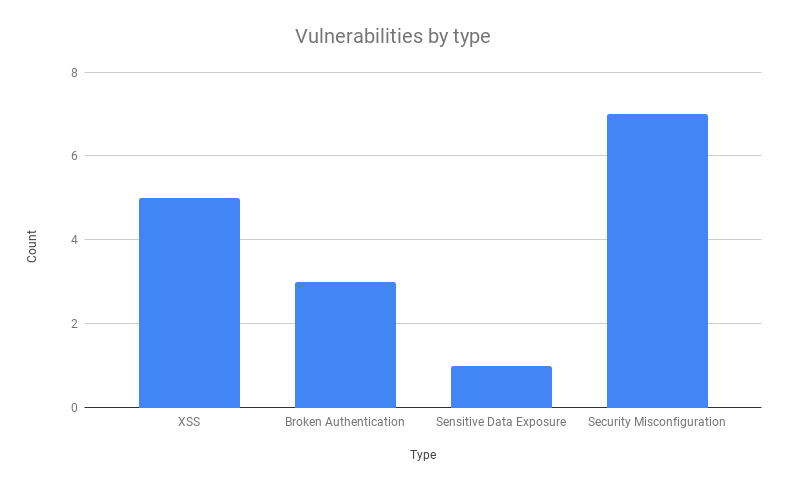
\includegraphics[width=0.6\textwidth]{img/vulns-by-type.png}
	\caption{Vulnerabilities by Type}
	\label{fig:vuln-by-type}
\end{figure}

In this part add a short summary of all vulnerabilities in non-technical terms.

It's also good to mention an estimation of efforts required to resolve the issues.